\section{Discussion}


\subsection{Trace metrics identify the mechanism}
Table~\ref{tab:trace} reports process counters for the \tb trajectories in the held-out paired set. The columns should be read as follows: ``Global'' is the average number of broad graph-search calls, ``Neigh.'' is the average number of one-hop neighborhood exploration calls, ``Zero'' is the average number of tool calls returning no useful candidate, ``Repeat'' is the average number of repeated or near-duplicate calls, ``Events'' is the average number of logged trace events, and ``Steps'' is the average controller step count. These counters reveal that \tb often spends substantial budget on exploration that does not translate into better ranking.

\begin{table}[t]
\centering
\caption{\textbf{Trace counters for \tb on held-out paired examples.} All entries are per-query averages. Higher values are not inherently better, they only indicate more interaction budget consumed before final ranking.}
\label{tab:trace}
\resizebox{\columnwidth}{!}{%
\begin{tabular}{lrrrrrr}
\toprule
Graph & Global & Neigh. & Zero & Repeat & Events & Steps \\
\midrule
PRIME & 4.1478 & 5.7010 & 4.6151 & 1.6564 & 11.8179 & 8.2577 \\
MAG & 2.4133 & 5.0200 & 2.2767 & 0.6633 & 9.8333 & 5.8667 \\
Amazon & 2.4040 & 5.4815 & 3.9293 & 0.6364 & 10.3131 & 6.1111 \\
\bottomrule
\end{tabular}}
\end{table}

The repeated-call counter is especially informative. Figure~\ref{fig:repeat_delta} conditions paired \mrr deltas on whether a \tb trajectory contains any repeated call. Each bar is the mean \tb-minus-unconditioned \mrr delta for a graph and bucket. PRIME is almost neutral when no repeated call occurs (-.0023), but becomes substantially worse when repetition appears (-.1228). MAG is negative in both buckets, yet repetition makes the degradation larger. The result suggests that repetition is not only an efficiency problem; it is a symptom of a controller that has lost the evidence trail.

\begin{figure}[t]
\centering
\resizebox{\columnwidth}{!}{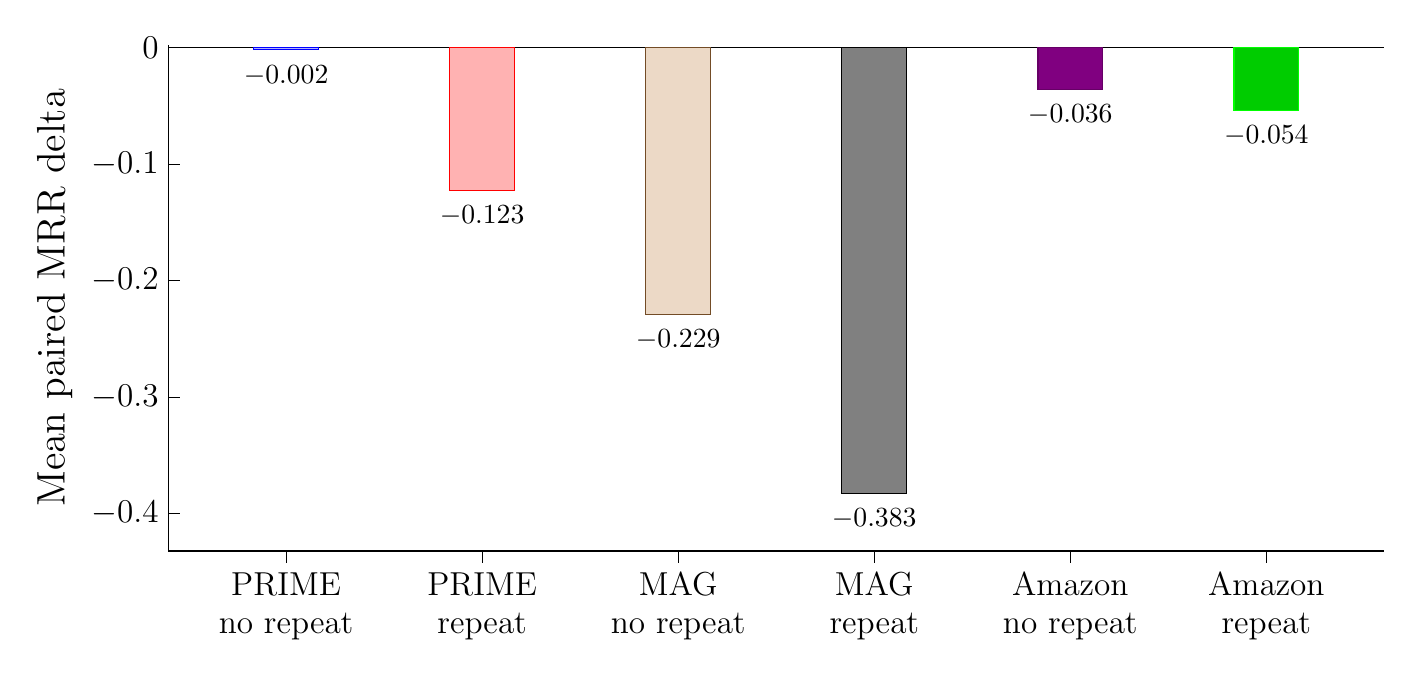
\begin{tikzpicture}
\begin{axis}[
    width=6.7in,
    height=3.15in,
    ybar,
    bar width=0.82cm,
    every axis plot/.append style={bar shift=0pt},
    ymin=-0.432,
    ymax=0.002,
    ylabel={Mean paired MRR delta},
    xtick={1,2,3,4,5,6},
    xticklabels={
        {PRIME\\no repeat},
        {PRIME\\repeat},
        {MAG\\no repeat},
        {MAG\\repeat},
        {Amazon\\no repeat},
        {Amazon\\repeat}
    },
    xticklabel style={align=center,font=\large},
    xmin=0.4,
    xmax=6.6,
    ytick={0,-0.1,-0.2,-0.3,-0.4},
    tick label style={font=\large},
    label style={font=\Large},
    title style={font=\LARGE},
    axis x line*=bottom,
    axis y line*=left,
    axis line style={black,semithick},
    tick style={black},
    extra y ticks={0},
    extra y tick labels={},
    extra y tick style={
        grid=major,
        major grid style={black,semithick},
        tick style={draw=none}
    },
    nodes near coords={
        \pgfmathprintnumber[fixed,precision=3,zerofill]{\pgfplotspointmeta}
    },
    point meta=rawy,
    every node near coord/.append style={
        font=\normalsize,
        black,
        anchor=north,
        yshift=-2pt
    },
    clip=false,
]

\addplot+[] coordinates {(1,-0.002)};
\addplot+[] coordinates {(2,-0.123)};
\addplot+[] coordinates {(3,-0.229)};
\addplot+[] coordinates {(4,-0.383)};
\addplot+[] coordinates {(5,-0.036)};
\addplot+[] coordinates {(6,-0.054)};

\end{axis}
\end{tikzpicture}
}
\caption{\textbf{Conditional rank loss by repeated-call bucket.} Each bar is the mean paired \mrr delta, \tb minus unconditioned. Here, ``repeat'' means at least one repeated or near-duplicate call occurred. Repetition predicts a larger loss on PRIME and MAG, and does not help on Amazon either.}
\label{fig:repeat_delta}
\end{figure}

\subsection{A tighter budget is not sufficient}
The constrained-budget probe asks whether \tb fails simply because it explores too long. Table~\ref{tab:budget} lowers the interaction budget and caps the number of global and neighborhood calls. The ``Steps'' column confirms that the probe shortens trajectories, but the rank metrics remain weak. This separates two hypotheses. If the main failure were only excessive length, tighter budgets should recover most of the unconditioned performance. Instead, the controller remains inaccurate, indicating that the problem is action selection for when to anchor, when to traverse, when to relax, and when to stop.

\subsection{Why the result matters}
The important finding is not simply that a prompt-level intervention failed. It is that the failure is structured and measurable. TraceBound changes the retrieval trajectory in ways that can be audited by showing how repeated calls indicate stagnation, zero-result calls indicate failed anchoring or traversal, and high exploration counts indicate budget spent without rank improvement. These are exactly the kinds of failures that final retrieval metrics can hide. This matters for adaptive graph retrieval because errors compound over the trajectory. A wrong early anchor can send the controller into a plausible but irrelevant neighborhood. A trace hint can then make the system more active around that bad anchor rather than causing a clean reset. In this setting, more explicit reasoning does not automatically produce better retrieval, instead it only creates more state for the controller to manage. The practical lesson is that profile and trace information should not be treated as globally useful context. They should be inputs to a calibrated action policy that decides when to search broadly, traverse locally, relax constraints, rerank, stop, or restart. TraceBound is therefore useful not because it improves the controller directly, but because it exposes the failure signals that a better controller must learn to act on.

\subsection{Failure taxonomy and corrective policy targets}
The trace counters support a taxonomy of operational failures. Table~\ref{tab:taxonomy} lists the failure class, the observable trigger, its likely ranking effect, and the policy correction suggested by the result. The final column is intentionally framed as a policy target rather than a prompt instruction. The experiments show that simply telling the controller about a failure symptom is insufficient; the system must learn when the symptom should change the next retrieval action.



\subsection{Design implications}
The study suggests three concrete design principles. First, a profile should be treated as an uncertain signal, not as privileged context. A controller should be able to ignore it when graph constraints are sufficient. Second, trace feedback should be gated by failure confidence. Repetition and empty calls are useful symptoms, but reacting too early can interrupt a correct path. Third, stopping should be a learned action. A system that only searches or explores will keep consuming budget even after the marginal value of another call is low.



\subsection{Implications for personalization}
The query profile in \tb is not a real user model, but it plays the same architectural role as a user profile would play in a personalized retriever - compact context injected before evidence is fetched. The negative result therefore gives a useful warning. Personalization should not be globally concatenated to every retrieval decision. Instead, the controller should learn a conditional policy which uses the profile when it helps disambiguate intent or rank candidates, ignores it when graph constraints dominate, and backtracks when profile-guided expansion enters an empty branch. In other words, personalization is not only a representation problem, it is a control problem over retrieval actions.
